\subsection{Middleware robótico: ROS 1 y ROS 2}
\label{sec:middleware_robotico_ros1_ros2}

El desarrollo de sistemas robóticos modernos requiere de software capaz de gestionar la interoperabilidad entre componentes heterogéneos. En este contexto, los \textit{middleware} robóticos proporcionan una capa de abstracción que facilita la integración de elementos dentro de una arquitectura modular. Entre las distintas soluciones propuestas, \gls{ros} se ha consolidado como uno de los marcos de desarrollo más utilizados en investigación y aplicaciones robóticas.

\gls{ros} proporciona un conjunto de herramientas y bibliotecas para la construcción de aplicaciones robóticas mediante la orquestación de módulos independientes denominados \textit{nodes}. Estos nodos intercambian información a través de un modelo de comunicación basado en el paradigma \textit{publish–subscribe}, en el que los productores de datos publican información en canales denominados \textit{topics}, mientras que los consumidores se suscriben a dichos canales para recibir los mensajes correspondientes. Este modelo facilita el desacoplamiento entre los distintos componentes del sistema y permite desarrollar arquitecturas robóticas distribuidas \cite{ros_concepts}. La figura \ref{fig:ros_basic_concepts} muestra la relación  de estos elementos.

\begin{figure}[H]
    \centering
    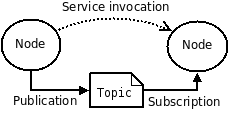
\includegraphics[width=0.35\linewidth]{figures/ROS_basic_concepts.png}
    \caption{Interacción entre elementos de ROS \cite{ros_concepts}}
    \label{fig:ros_basic_concepts}
\end{figure}

La primera generación del sistema, conocida como \gls{ros1}, la comunicación entre nodos se implementa mediante mecanismos de transporte basados en los protocolos de red \gls{tcp} y \gls{udp}, a través de las implementaciones TCPROS y UDPROS. Aunque esta arquitectura ha demostrado ser eficaz, presenta ciertas limitaciones en términos de escalabilidad y soporte para aplicaciones con requisitos estrictos de tiempo real. En particular, la latencia de comunicación entre nodos puede verse afectada por factores como el tamaño de los mensajes, la carga del sistema o las características de la red subyacente \cite{nishimura2021raplet}.

Con el objetivo de superar estas limitaciones, la segunda generación del \textit{framework}, \gls{ros2}, introduce una arquitectura de comunicación basada en el estándar \gls{dds}. Este middleware, orientado a sistemas distribuidos, implementa de forma nativa el modelo \textit{publish--subscribe} y proporciona mecanismos avanzados de gestión de políticas de \gls{qos}, como la configuración de políticas de latencia \cite{ros_concepts}. La adopción de \gls{dds} permite así mejorar la escalabilidad de los sistemas robóticos y facilita su integración en entornos distribuidos complejos, al tiempo que posibilita adaptar el comportamiento de la comunicación a los requisitos específicos de cada aplicación.

En consecuencia, el uso de \gls{ros2} es adecuado para el desarrollo de sistemas robóticos distribuidos. No obstante, el comportamiento temporal de estos sistemas depende de múltiples factores, incluyendo la configuración del middleware, la carga computacional de los nodos y las características de la red de comunicaciones. Por ello, el análisis del rendimiento y de la latencia en sistemas robóticos basados en ROS constituye un aspecto fundamental en el diseño y evaluación de arquitecturas robóticas distribuidas. Los avances en este área se tratan en la siguiente sección \ref{sec:evaluacion_de_latencia_en_sistemas_roboticos_distribuidos}.